\documentclass{beamer}
\usepackage[utf8]{inputenc}
\usetheme{Warsaw}%{Berkeley} Madrid
\usecolortheme{Dolphin} %dolphin, lily, orchid, structure sidebartab wolverine crane
\title[Conception et adaptation de Serious Games]{Serious games pour la santé :\\ Méthodologie de conception et adaptation de la difficulté}
\author{MÉLIA Geoffrey - Master 2 Informatique}
\institute{Université Montpellier II - NaturalPad}
\date{05 septembre 2013}

%\addtobeamertemplate{footline}{\hfill\insertframenumber/\inserttotalframenumber\hspace{2em}\null}

\AtBeginSection[]
{
\begin{frame}
\tableofcontents[currentsection,hideallsubsections]
\end{frame}
}

\begin{document}
	\setbeamertemplate{navigation symbols}{} % supprimer les symboles de navigation
	%\setbeamercovered{dynamic} permet de griser les éléments en attente de \pause
	\addtobeamertemplate{footline}{\hfill\insertframenumber/\inserttotalframenumber}
%	\addtobeamertemplate{footline}
%	{
%		\begin{beamercolorbox}[wd=.2\paperwidth,ht=2.25ex,dp=1ex,right]{section in head/foot}%
%			\usebeamerfont{section in head/foot}
%			\insertframenumber{} / \inserttotalframenumber\hspace*{2ex}
%		\end{beamercolorbox}%
%	}
		
	\begin{frame}
		\titlepage
	\end{frame}
	
	%Slide d'intro avant le plan
	\begin{frame}{Avant-propos}
		\begin{block}{NaturalPad}
			L'informatique au service de la santé.
		\end{block}		
		\begin{block}{Objectif}
			Adapter la difficulté d'un jeu pour la santé.
		\end{block}		
	\end{frame}
	
	%Plan
	\begin{frame}{Plan}
		\tableofcontents
	\end{frame}
	
	\section{Introduction}
		
		\begin{frame}{NaturalPad}
			\begin{block}{Une SSII dans le secteur de la santé}
				Expert NTIC Santé auprès des Centres Hospitaliers et personnels soignants.\\
				Développeur de serious games à but thérapeutiques.
			\end{block}
			
			\begin{figure}
				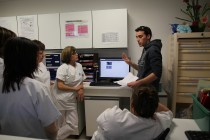
\includegraphics[width=5cm]{../images/formation.jpg}
				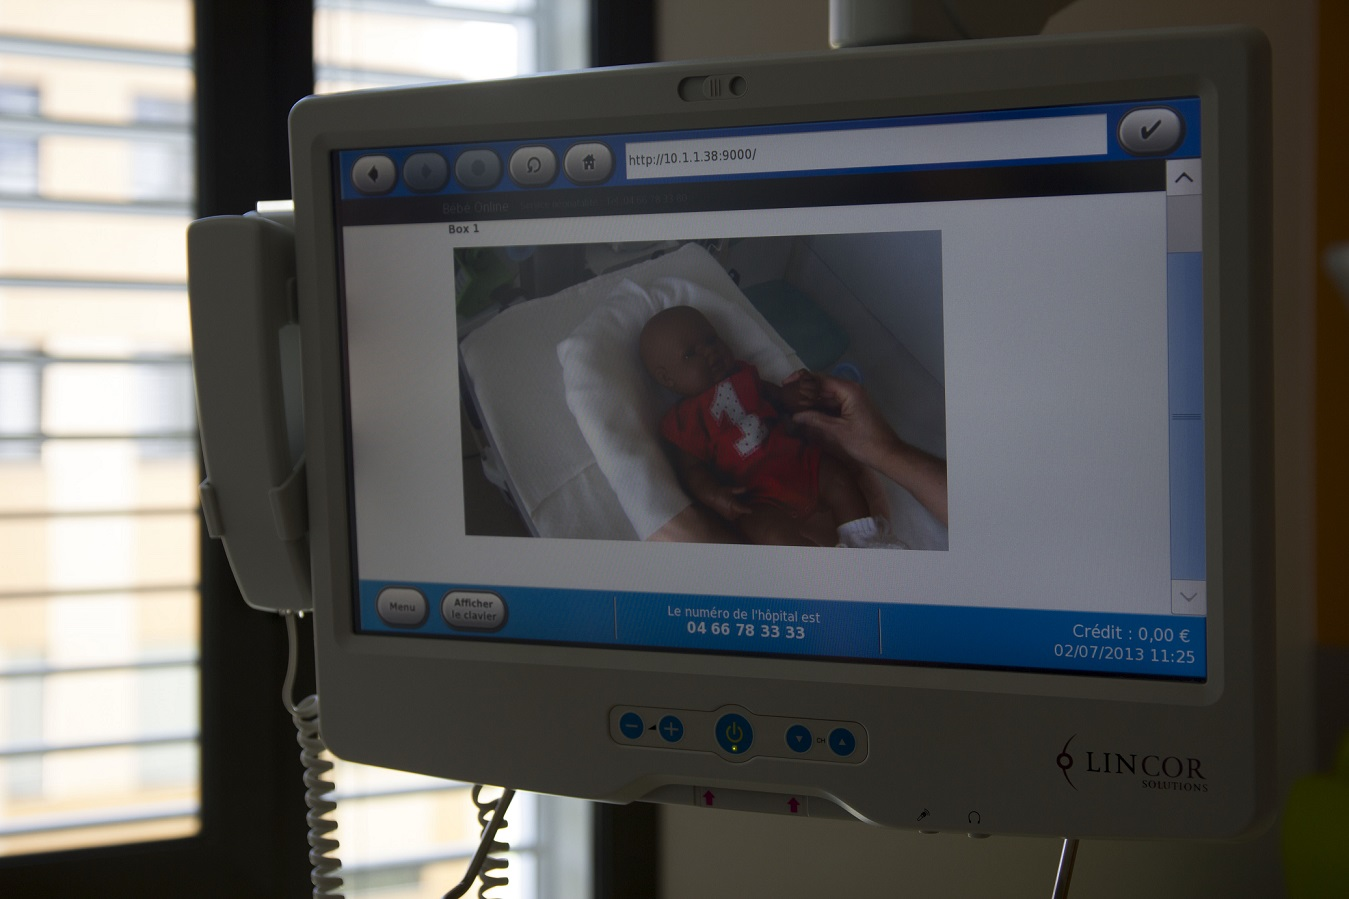
\includegraphics[width=5cm]{../images/bebeonline.jpg}		
				%\caption{A gauche : Formation du personnel médical aux outils déployés. A droite : Terminal avec BebeOnline}	
			\end{figure}
		\end{frame}	
	
		\begin{frame}{Hammer \& Planks}
			\begin{block}{Un serious game pour la santé}
				• Un jeu vidéo sérieux d'aide à la réhabilitation motrice.\\
				• Adapté aux personnes hémiplégiques : équilibre, membres supérieurs et tronc.
			\end{block}
			
			\begin{figure}
				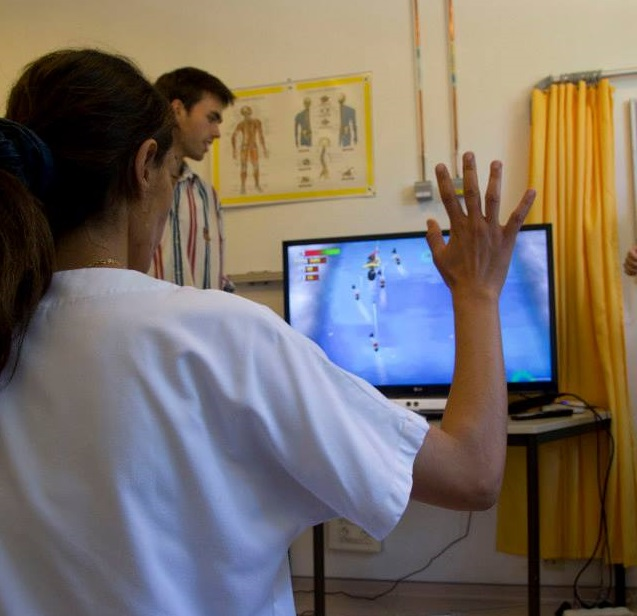
\includegraphics[width=5cm]{../images/test_lapeyronie_2.png}
			\end{figure}
		\end{frame}	
		
		\begin{frame}{Travail d'étude et de recherche : \emph{ZigFugl Meyer}}
			\begin{minipage}{0.40\linewidth}
				\begin{figure}
					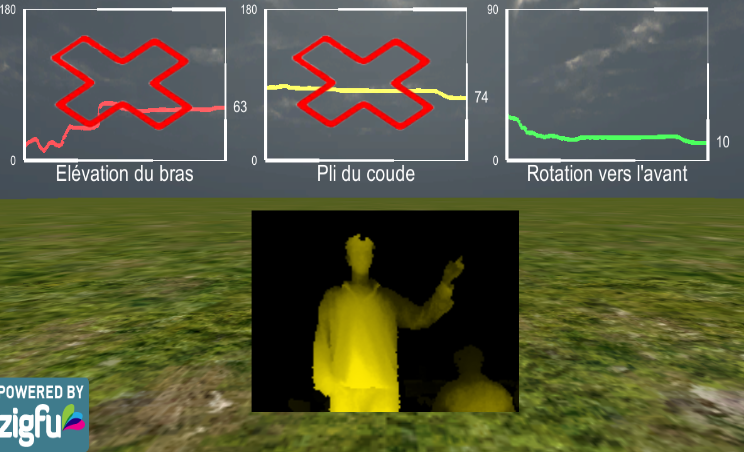
\includegraphics[width=4.2cm]{../images/zigfugl-meyer_1.png}\\
					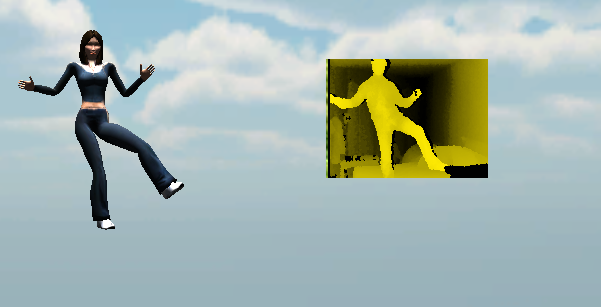
\includegraphics[width=4.2cm]{../images/zigfugl-meyer_2.png}
				\end{figure}
			\end{minipage}
			\begin{minipage}{6cm}%{0.55\linewidth}
				Utilisation de l'informatique pour l'évaluation de capacités motrices (Fugl Meyer assessment). 
					\begin{itemize}
						\item Utilisation de la Kinect comme interface naturelle.
						\item Expérimentation d'une gamification du test.
						\item Vérification automatique de la réussite de l'exercice.
					\end{itemize}
			\end{minipage}
		\end{frame}
	
	\section{Problématique et Objectifs}
		\begin{frame}{Serious Games}
			\begin{block}{Qu'est-ce que c'est?}
				Application qui combine une intention sérieuse à des ressorts ludiques.
			\end{block}\pause
			\begin{exampleblock}{Utilisés dans :}
				Éducation, formation, entraînement, marketing, communication, santé.
			\end{exampleblock}	\pause
			\begin{alertblock}{Ne pas confondre}
				Serious Game et Serious Gaming
			\end{alertblock}
		\end{frame}
	
		\begin{frame}{Serious Games pour la rééducation}
			\begin{exampleblock}{Objectifs et qualités}
				- renforcer la motivation des patients.\\
				- oublier que c'est du travail. \\
				- augmenter le temps de travail.
			\end{exampleblock}\pause
			\begin{alertblock}{Un problème d'adaptation}
			Il est nécessaire de prendre en compte :\\
					- la pathologie et les capacités physiques du patient.\\
					- les objectifs et contraintes thérapeutiques.\\
					- son âge, son aisance avec les nouvelles technologies.\\
					- son niveau de joueur.
			\end{alertblock}
		\end{frame}
	
		\begin{frame}{Objectifs de stage}		
			\large{Comment proposer des jeux vidéo pour la santé adaptés?}
		\end{frame}
		
	\section{Proposition et réalisations}	
		\begin{frame}
			\begin{block}{Axes de travail}			
				\begin{itemize}
					\item Ajuster les paramètres de H\&P via l'interface thérapeute.\\
					\item Proposition d'outils d'aide à la conception de jeux pour la santé.\\
					\item Suggestion d'une méthodologie de conception.
				\end{itemize}
			\end{block}
		\end{frame}		
			
		\begin{frame}{Interface thérapeutique}
			\begin{block}{}
				• Avoir un accès commun et direct aux paramètres ajustables.\\
				• Classer les paramètres et ajuster les plages de valeurs possibles.\\
				• Ajuster le jeu en direct en fonction des besoins.\\
				• Utiliser des fichiers de configuration pour enregistrer des sets de valeurs.
			\end{block}
			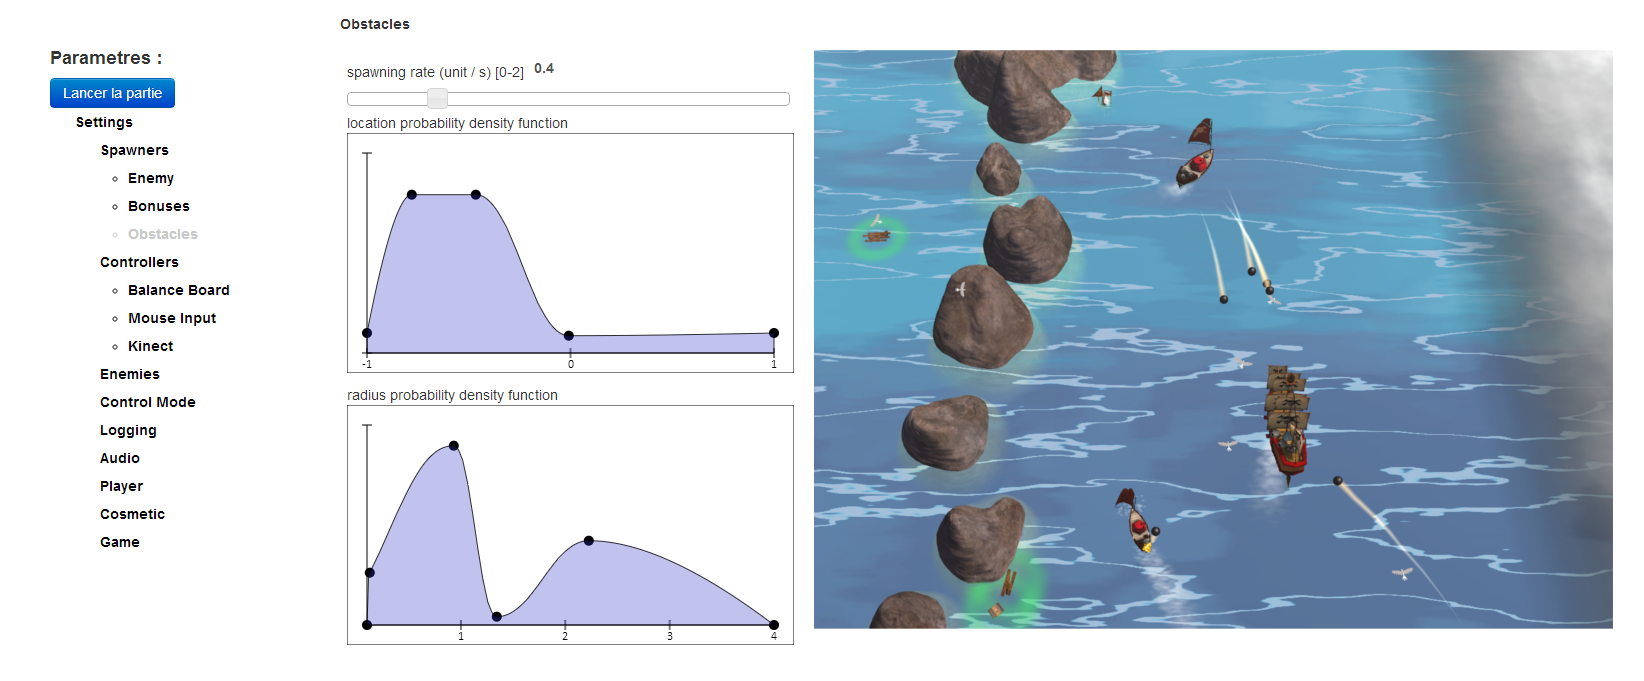
\includegraphics[width=10cm, height=4cm]{../images/comparatif_interface_rochers.png}		
		\end{frame}			
		
		\begin{frame}{Aide à la conception de jeux sérieux pour la santé}
			\begin{block}{Acquisition des connaissances préalables}
				Analyse de l'existant.\\
				Connaissances médicales et enjeux thérapeutiques.\\
				Exploration des théories utiles aux SG.				
			\end{block}
		\end{frame}
	
		\begin{frame}
			- interface thérapeutique et ajustement des paramètres
			- méthodo de conception participative
			- conception lombalgie, verticalisation
			- poursuite du travail de TER : fugl meyer informatique
		\end{frame}
	
	\section{Perspectives}
		\begin{frame}
		
		\end{frame}
	
	\section{Conclusion}
		\begin{frame}
		
		\end{frame}

\end{document}